\section{Audio: Speech Recognition and Audio Classification}
\label{sec:annex-18}

\subsection{Executive Summary}

\texttt{frankenstein\_audio} is the fourth model class of the toolkit. It owns an audio frontend---log-mel filterbanks or a raw spectrogram, optional SpecAugment \citep{Park2019}, and two stride-2 convolutions that reduce the frame rate by $4\times$---and then runs the same \texttt{HybridLayer} stack as the text encoder over the resulting frame sequence. Because the stack is modality-agnostic, every sequence mixer (including the Conformer of Appendix~\ref{sec:annex-17}), normalization, residual strategy, positional encoding, optimizer and routing block is available unchanged. The class supports two tasks: \textbf{automatic speech recognition} (\texttt{asr}, with a CTC \citep{Graves2006ctc} or an RNN-Transducer \citep{Graves2012} loss) and \textbf{audio classification} (\texttt{audio\_classification}, clip-level cross-entropy). The same frontend, driven with \texttt{audio.feature: raw}, accepts multichannel one-dimensional sensor signals such as EEG, EMG or accelerometer traces for classification.

The reference recipe is the Conformer frontend of \citet{Gulati2020}: 80-channel log-mel filterbanks with a 25\,ms window and a 10\,ms stride, two $3\times3$ convolutions with stride 2, a linear projection to the model width, and SpecAugment with frequency width $F=27$, ten time masks and a maximum time-mask ratio $p_S = 0.05$. The three reference sizes (S/M/L) are reproduced in Table~\ref{tab:audio-sizes}.

\subsection{The \texttt{frankenstein\_audio} Model Class}

\begin{figure}[H]
\centering
\fitfigure{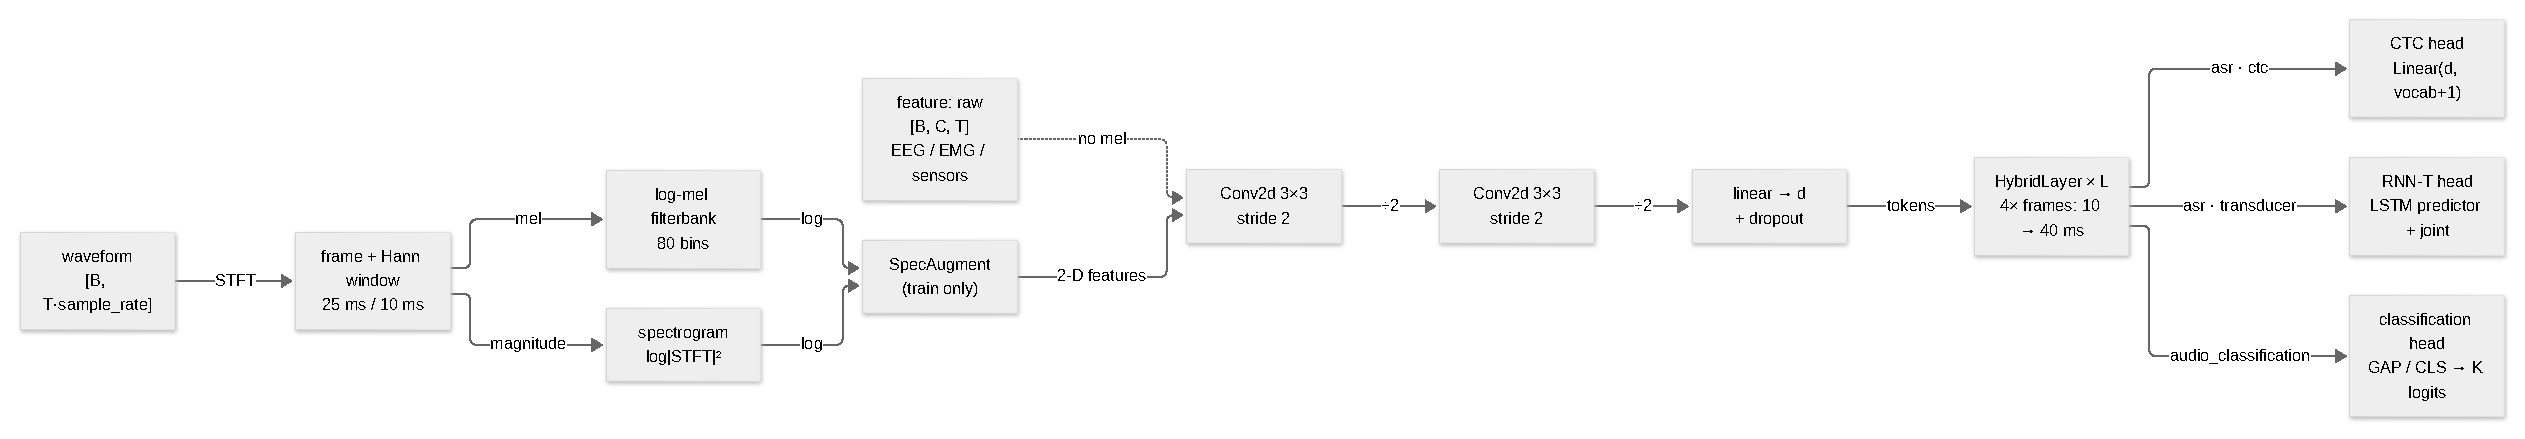
\includegraphics{figures/audio_frontend.pdf}}
\caption{Dataflow of the audio frontend: waveform $\to$ 25\,ms/10\,ms framing $\to$ 80-bin log-mel (or spectrogram, or raw multichannel frames) $\to$ SpecAugment (training only) $\to$ two stride-2 Conv2d stages ($4\times$) $\to$ linear projection $\to$ \texttt{HybridLayer} stack $\to$ CTC, RNN-T or classification head.}
\label{fig:audio-frontend}
\end{figure}

\subsubsection{Audio Frontend}

The frontend module turns a batch of waveforms $w \in \mathbb{R}^{B \times T}$ (or a batch of multichannel clips $w \in \mathbb{R}^{B \times C \times T}$ in \texttt{raw} mode) into a feature map:

\begin{enumerate}[leftmargin=*]
    \item \textbf{Framing:} the waveform is cut into overlapping windows of \texttt{window\_ms} $=25$\,ms every \texttt{stride\_ms} $=10$\,ms, with a Hann window, at \texttt{sample\_rate} $=16000$\,Hz. At the reference rate this yields frames of 400 samples with a 160-sample hop, i.e.\ 100 frames per second.
    \item \textbf{Spectral representation} (\texttt{audio.feature}):
    \begin{itemize}[leftmargin=*]
        \item \texttt{logmel} (default): an $80$-bin mel filterbank (Equation~\ref{eq:audio-mel}) followed by a log compression;
        \item \texttt{spectrogram}: $\log|\mathrm{STFT}(w)|^2$ with no mel projection;
        \item \texttt{raw}: no spectral transform; the clip is fed as a $C \times T$ map (Section~\ref{sec:annex-18-eeg}).
    \end{itemize}
    \item \textbf{SpecAugment} \citep{Park2019}: $F$ frequency channels are masked per clip, and up to \texttt{time\_masks} time bands of width at most $p_S \cdot T$ are masked, both with zero fill (training only).
\end{enumerate}

The mel filterbank is
\begin{equation}
M_k(f) = \max\Big(0,\ \min\Big(\tfrac{f-f_{k-1}}{f_k-f_{k-1}},\ \tfrac{f_{k+1}-f}{f_{k+1}-f_k}\Big)\Big),
\label{eq:audio-filterbank}
\end{equation}
for $K = 80$ triangular filters spaced on the mel scale, $\mathrm{mel}(f) = 2595 \log_{10}(1 + f/700)$, and the log-mel feature is
\begin{equation}
x_k = \log\Big(\sum_{f} M_k(f)\,|X(f)|^2 + \epsilon\Big).
\label{eq:audio-mel}
\end{equation} When \texttt{torchaudio} is importable, the frontend uses \texttt{torchaudio.transforms.MelSpectrogram} for Equation~\ref{eq:audio-mel}; otherwise it falls back to a pure-PyTorch implementation built on \texttt{torch.stft} and a cached filterbank matrix. The two paths are numerically equivalent up to filterbank convention (HTK vs.\ Slaney mel spacing), and the pure-PyTorch path is what keeps CPU-only CI free of the optional \texttt{audio} extra.

\subsubsection{Convolutional Subsampling}

Two convolutional stages reduce the frame rate by $4\times$ (10\,ms $\to$ 40\,ms), which is what makes a 30-second utterance a $\sim$750-token sequence instead of 3000:
\begin{equation}
F = \mathrm{Dropout}\Big(W_p\,\mathrm{Conv2d}_{3\times3,\,s=2}\big(\mathrm{Conv2d}_{3\times3,\,s=2}(X)\big)\Big),
\qquad W_p \in \mathbb{R}^{d \times d_c},
\label{eq:audio-subsampling}
\end{equation}
where $X$ is the $\texttt{n\_mels} \times T'$ feature map with \texttt{conv\_channels} channels after the first stage, and $W_p$ projects the flattened channels to the model width $d$. Both stages are fixed at $3\times3$ kernels with stride 2; \texttt{audio.conv\_channels} (32) sets the channel width of the first stage and \texttt{audio.n\_fft} (400) the STFT size.

\subsubsection{Forced Encoder Mode and the HybridLayer Stack}

\texttt{frankenstein\_audio} forces \texttt{mode: encoder}, exactly as \texttt{frankenstein\_vit} does: the audio tasks are bidirectional (a CTC or transducer encoder must see both past and future frames), and the Conformer's convolution padding is symmetric in encoder mode. The class mirrors the ViT wrapper pattern---frontend, \texttt{HybridLayer} stack, task head---and its layer loop keeps the same hooks, so AttnRes, mHC, Hyperloop, looped depth, MoE, Mixture-of-Depths and BitNet all work without audio-specific code. All task heads are built after the final normalization:

\begin{itemize}[leftmargin=*]
    \item \textbf{CTC:} $\mathrm{Linear}(d, V+1)$ over the frame sequence, where the extra class is the blank.
    \item \textbf{RNN-T:} a one-layer LSTM prediction network over the previous non-blank labels (\texttt{audio.asr\_decoder\_dim}, \texttt{asr\_decoder\_layers}, \texttt{asr\_decoder\_dropout}), and a joint network $z_{t,u} = \tanh(W_e h_t + W_p h_u + b)$, $\mathrm{logits}_{t,u} = W_o z_{t,u}$.
    \item \textbf{Classification:} a pooled vector (global average pooling, or a learned \texttt{[CLS]} token prepended to the frame sequence, per \texttt{pooling\_mode}) projected to \texttt{num\_classes} logits.
\end{itemize}

\subsection{Automatic Speech Recognition}

\subsubsection{CTC}

Connectionist temporal classification \citep{Graves2006ctc} marginalizes over all frame-level alignments that collapse to the target label sequence $y$ under the many-to-one map $\mathcal{B}$ (merge repeats, delete blanks):
\begin{equation}
\mathcal{L}_{\text{CTC}} = -\log \sum_{\pi \in \mathcal{B}^{-1}(y)} \prod_{t=1}^{T} p(\pi_t \mid x),
\label{eq:audio-ctc}
\end{equation}
computed with \texttt{torch.nn.functional.ctc\_loss} in log space with \texttt{zero\_infinity=False}, so that impossible alignments do not poison the gradient.

\subsubsection{RNN-Transducer}

The RNN-T loss \citep{Graves2012} sums over \emph{label-and-blank} alignments on the $T \times (U+1)$ lattice. With $\alpha_{t,u}$ the log-probability of the prefix $y_{1:u}$ after $t$ encoder frames, the forward recursion is
\begin{equation}
\alpha_{t,u} = \operatorname{logsumexp}\Big(
\underbrace{\alpha_{t-1,u} + \log p(\varnothing \mid t-1, u)}_{\text{advance time}},
\;
\underbrace{\alpha_{t,u-1} + \log p(y_u \mid t, u-1)}_{\text{emit label}}
\Big),
\label{eq:audio-rnnt}
\end{equation}
with $\alpha_{0,0} = 0$ and $-\infty$ elsewhere, $p(\cdot \mid t,u) = \operatorname{softmax}(\mathrm{logits}_{t,u})$, and
\begin{equation}
\mathcal{L}_{\text{RNN-T}} = -\alpha_{T,U}.
\label{eq:audio-rnnt-loss}
\end{equation} The implementation is autograd-friendly in pure PyTorch (log-domain dynamic programming on the lattice, with the gradient obtained by the standard backward recursion), and takes the \texttt{torchaudio.functional.rnnt\_loss} fast path when the optional dependency is installed. The lattice is $O(T \cdot U)$ in memory, which is why the predictor is kept shallow (\texttt{audio.asr\_decoder\_layers}, default 1) and narrow (\texttt{audio.asr\_decoder\_dim}, default 320). The loss is selected with \texttt{audio.asr\_loss} (\texttt{ctc} by default).

\subsubsection{Decoding and Error Rate}

Greedy CTC decoding takes the per-frame argmax, collapses repeats and removes blanks. Greedy RNN-T decoding alternates a label emission with a frame advance until the blank is scored higher than the next label. Both are scored with the character error rate
\begin{equation}
\mathrm{CER} = \frac{S + D + I}{N},
\label{eq:audio-cer}
\end{equation}
where $S$, $D$, $I$ are the substitutions, deletions and insertions of the Levenshtein alignment against the reference transcript and $N$ is the reference length.

\subsection{Audio Classification}

Classification reuses the pooling and head conventions of the Vision Transformer (Appendix~\ref{sec:annex-vision}): \texttt{pooling\_mode: cls} prepends a learned token and reads position 0, \texttt{pooling\_mode: gap} (the default) averages the frame outputs. The head is a zero-initialized $\mathrm{Linear}(d, K)$ trained with cross-entropy and the same label smoothing knob as the vision tasks. SpecAugment applies to the feature map before subsampling, so it augments the input, never the token sequence.

\subsection{SpecAugment}

Following \citet{Park2019} in its ``LibriSpeech basic'' configuration, the two mask types are applied independently per clip:
\begin{equation}
\Delta f \sim \mathcal{U}[0, F], \quad f_0 \sim \mathcal{U}[0, \nu - \Delta f],
\qquad
\Delta t \sim \mathcal{U}[0, p_S \cdot T], \quad t_0 \sim \mathcal{U}[0, T - \Delta t],
\label{eq:audio-specaugment}
\end{equation}
with $F = 27$, \texttt{time\_masks} $= 10$ and $p_S = 0.05$, each mask zeroing a $\Delta f \times \Delta t$ rectangle. Time \emph{warping}, the third SpecAugment transform, is not implemented---it requires a per-sample warp of the time axis that interacts poorly with the fixed-length bucketing of the dataset. Frequency and time masking carry most of the regularization benefit in the paper's own ablations, and both are disabled at evaluation time.

\subsection{Reference Sizes}

\begin{table}[H]
\centering
\small
\begin{tabular}{L{2.3cm}cccccc}
\toprule
\textbf{Variant} & \textbf{Layers} & \textbf{$d$} & \textbf{Heads} & \textbf{Kernel} & \textbf{Params} & \textbf{RNN-T $d_{dec}$} \\
\midrule
Conformer-S & 16 & 144 & 4 & 32 & 10.3M & 320 \\
Conformer-M & 17 & 256 & 4 & 32 & 30.7M & 640 \\
Conformer-L & 17 & 512 & 8 & 32 & 118.8M & 640 \\
\bottomrule
\end{tabular}
\caption{Reference Conformer sizes of \citet{Gulati2020} (Table~1), which the example presets follow. The RNN-T decoder width is only used when \texttt{audio.asr\_loss: transducer}.}
\label{tab:audio-sizes}
\end{table}

\subsection{Example Configurations}

The ASR examples use \texttt{astroza/chilean-jokes-festival-de-vina} (Spanish audio at 16\,kHz with transcripts, 50 rows), a dataset small enough to run end-to-end on CPU as a smoke test. The classification example falls back to the synthetic \texttt{DummyAudioDataset} when no dataset is reachable.

\begin{verbatim}
model_class: frankenstein_audio
model:
  dims: {hidden_size: 144, num_layers: 16, num_heads: 4}
  dims.layer_pattern: [conformer_attn, ...]   # 16 entries
  attention.conformer: {kernel_size: 32, macaron: true, conv_norm: batch}
audio:
  feature: logmel
  sample_rate: 16000
  n_mels: 80
  window_ms: 25
  stride_ms: 10
  n_fft: 400
  conv_channels: 32
  asr_loss: ctc          # or transducer
  asr_decoder_dim: 320
  asr_decoder_layers: 1
  asr_decoder_dropout: 0.1
audio_dataset:
  dataset_name: astroza/chilean-jokes-festival-de-vina
  split: train
  audio_column: audio
  text_column: text
  spec_augment: {enabled: true, freq_mask_width: 27,
                 time_masks: 10, time_mask_ratio: 0.05}
training:
  task: asr
\end{verbatim}

\subsection{Generic 1-D Signals: EEG and Beyond}
\label{sec:annex-18-eeg}

The frontend is not tied to speech. With \texttt{audio.feature: raw}, the mel filterbank and SpecAugment are skipped and the clip is treated as a multichannel $C \times T$ map, with \texttt{audio.in\_channels: C}. The two stride-2 convolutions then act as a learned filter bank over time (and, as a side effect, over the channel axis), the linear projection produces $d$-wide tokens, and the \texttt{HybridLayer} stack sees a sequence of frames exactly as it does for speech. This makes the class usable, at least for \textbf{classification}, on:

\begin{itemize}[leftmargin=*]
    \item \textbf{EEG:} $C$ electrodes $\times$ $T$ samples per epoch, labelled with a cognitive state, sleep stage or pathology; electrodes play the role of the mel channels.
    \item \textbf{EMG / ECG / EDA:} one or a few channels, labelled with gesture, activity or anomaly class.
    \item \textbf{Accelerometer / IMU:} $C \in \{3, 6, 9\}$ axes, labelled with activity or device state.
    \item \textbf{Industrial and environmental sensors:} vibration, pressure, acoustic emission traces, labelled per window.
\end{itemize}

\paragraph{What carries over.} Everything downstream of the frontend: all 45 mixers (Conformer is a good default because its convolution branch matches the local morphology of biosignals), all 6 norms, AttnRes/mHC/MoE/MoD, the 23 optimizers, the frozen-encoder \texttt{text\_classification} recipe, and the checkpoint/deployment paths. Length bucketing, padding masks and the CER/CER-style evaluation are dataset-side and are unaffected by the modality.

\paragraph{Limitations.} Raw mode is a convenience, not a replacement for a domain frontend:
\begin{enumerate}[leftmargin=*]
    \item \textbf{Channel axis downsampling.} The two stride-2 \texttt{Conv2d} stages are fixed and halve both spatial axes, so a montage with fewer than four channels loses its channel axis entirely; keep $C \geq 4$ (or project the montage to a wider map first).
    \item \textbf{No montage geometry.} Electrode positions, referential vs.\ bipolar montages and inter-channel correlations are not encoded; the convolution sees channels as an unordered stack, unlike EEG-specific models with topographic or graph priors.
    \item \textbf{No spectral prior.} \texttt{logmel} and \texttt{spectrogram} assume audio band limits and mel spacing that do not apply below 20\,Hz or above 8\,kHz; raw mode avoids the mismatch but also loses the band-aligned inductive bias.
    \item \textbf{Classification only.} CTC and RNN-T require a token-level target sequence. Sequence-to-sequence labelling of sensor windows (e.g.\ sleep-stage sequences) is out of scope; use per-window classification and a post-hoc decoder instead.
    \item \textbf{Statistics and normalization.} The convolution module's BatchNorm uses per-batch statistics; for EEG the amplitude scale varies by subject and session, so per-channel normalization in the dataset is recommended over relying on the frontend.
    \item \textbf{Sampling-rate assumptions.} \texttt{sample\_rate} is used to convert \texttt{window\_ms}/\texttt{stride\_ms} into samples; for raw signals set it to the true acquisition rate and choose the window in milliseconds accordingly.
\end{enumerate}

\subsection{PyTorch Pseudocode}

\begin{algorithmic}[1]
\State \textbf{Input:} waveforms $w$, lengths $\ell$, transcripts $y$ (ASR) or labels $c$ (classification)
\State $F \gets \texttt{frontend}(w)$ \Comment{log-mel / spectrogram / raw, $(B, C, 80, T')$}
\State $F \gets \texttt{spec\_augment}(F)$ \Comment{training only}
\State $F \gets \texttt{conv2d}_{3\times3, s=2}(F)$; \quad $F \gets \texttt{conv2d}_{3\times3, s=2}(F)$
\State $x \gets \texttt{dropout}(\texttt{linear}(F))$ \Comment{$(B, T'/4, d)$ tokens}
\State $x \gets x + \texttt{pos\_encoder}(x)$ \Comment{frame positions, not mel bins}
\For{each \texttt{layer} in \texttt{layers}}
    \State $x \gets \texttt{layer}(x)$ \Comment{\texttt{HybridLayer}, forced encoder mode}
\EndFor
\State $x \gets \texttt{final\_norm}(x)$
\If{task $=$ asr and loss $=$ ctc}
    \State $\mathrm{logits} \gets \texttt{ctc\_head}(x)$; \quad $\mathcal{L} \gets \texttt{ctc\_loss}(\log\mathrm{softmax}(\mathrm{logits}), y, \ell/4)$
\ElsIf{task $=$ asr and loss $=$ transducer}
    \State $h^{pred} \gets \texttt{predictor}(y)$; \quad $\mathrm{logits}_{t,u} \gets \texttt{joint}(x_t, h^{pred}_u)$
    \State $\mathcal{L} \gets \texttt{rnnt\_loss}(\mathrm{logits}, y, \ell/4)$
\Else
    \State $\mathrm{logits} \gets \texttt{class\_head}(\texttt{pool}(x))$; \quad $\mathcal{L} \gets \mathrm{CE}(\mathrm{logits}, c)$
\EndIf
\end{algorithmic}

\subsection{Deviations and Implementation Notes}

\begin{itemize}[leftmargin=*]
    \item \textbf{Optional torchaudio.} The frontend prefers \texttt{torchaudio.transforms} but never requires it; the pure-PyTorch fallback keeps the CPU CI and the \texttt{cpu} extra torchaudio-free (decision D7 of the architecture guide).
    \item \textbf{Time warping.} Not implemented (Equation~\ref{eq:audio-specaugment} covers frequency and time masking only); time warping is the transform the paper uses least.
    \item \textbf{Shallow predictor.} The RNN-T prediction network is a single LSTM layer by default (\texttt{audio.asr\_decoder\_layers}), trading the paper's deeper predictor for an $O(T \cdot U)$ lattice that fits in memory at the reference batch sizes.
    \item \textbf{Export.} The HuggingFace and GGUF exports reject audio artifacts explicitly, as they do for SBERT: there is no upstream \texttt{FrankensteinForAudioClassification} mapping. \texttt{deploy --format standard|quantized} works unchanged.
    \item \textbf{Cache.} There is no incremental encoder cache for audio; ASR consumes a whole utterance per forward.
\end{itemize}
